\documentclass[UTF8]{ctexart}
\usepackage{titlesec}
\usepackage{fancyhdr}
\usepackage{geometry}
\usepackage{listings}
\usepackage{xcolor}
\usepackage{graphicx}
\usepackage{amsmath}  % 提供了高级数学公式环境
\usepackage{amsfonts} % 提供数学字体
\usepackage{amssymb}  % 提供额外的数学符号

\geometry{left=1.0in,right=1.0in,top=0.3in,bottom=0.3in}

\pagestyle{fancy}
\fancyhf{} % 清空当前的页眉和页脚
\fancyfoot[C]{\thepage} % 页脚中间显示页码

\ctexset{
    section={%
        format=\raggedright\Large\bfseries,
        afterskip=10pt,
    },
    subsection={%
        format=\raggedright\normalsize,
        afterskip=8pt,
    }
}

\lstset{
    language=C++, 
    basicstyle=\ttfamily\small, % 字体样式和大小
    keywordstyle=\color{blue}, % 关键字颜色
    commentstyle=\color{gray}, % 注释颜色
    stringstyle=\color{red}, % 字符串颜色
    numbers=left, % 显示行号
    numberstyle=\tiny\color{gray}, % 行号样式
    frame=single, % 代码框
    breaklines=true, % 自动换行
    captionpos=b % 标题位置
}


\begin{document}

\title{\vspace{0cm}钢条切割实验报告}
\author{程远2234412848}
\date{}
\maketitle
\tableofcontents
\newpage

\section{问题描述}
设有一个长度为L的钢条,在钢条上标有n个位置点(p1,p2,…,pn)。
现在需要按钢条上标注的位置将钢条切割为n+1段,假定每次切割所需要的代价与所切割的钢条长度成正比。
现需要编写一个算法,能够确定一个切割方案,使切割的总代价最小。

\section{问题分析}
此问题与课本50页的矩阵连乘问题非常相似,可以用类似的方法解决。矩阵连乘问题中,切割成本为$p_{i-1} * p_k * p_j$
而在本题中,切割成本为$j - i$。要想总切割成本最少,应该要使得在切割方案中,尽可能避免切割长钢条,以减少总切割代价。
而切割问题显然具有最优子结构的特征,可以分解为一系列子问题,每个子问题求解一个较小区间的最小切割代价,当所有子问题最优时,
总问题也达到最优,具体算法设计见下一部分。

\section{算法设计}
\subsection{状态定义}
为了找到最优切割方案,需要对切割过程进行拆解,定义每一段的最小代价:
令points数组记录所有的切割点的位置,其中$points[0]$和$points[n+1]$分别表示钢条的起始点和终点。
由题目定义可知,$points[0] = 0, points[n+1] = L$
设$m[i][j]$表示将钢条从$points[i]$到$points[j]$切割的最小代价。

\subsection{最优子结构}
该问题的最优子结构在于,对于每一个区间$[i,j]$的切割位置,可以将其分解为若干子区间的最优解。具体而言,如果我们在 
$[i,j]$之间选择某个切割位置$breakPoint$,那么总代价为
\[
m[i][j] = m[i][breakPoint] + m[breakPoint][j] + points[j] - points[i]
\]

\subsection{重叠子问题}
该问题分解为一系列子问题之后,不难发现不同的子问题之间有所重叠。例如,计算$[k,k+5]$区间的最小代价与计算$[k-1,k+6]$区间的最小代价
都涉及到计算$[k,k+5]$区间的最小代价。因此,子区间切割代价的计算会多次重复。通过动态规划,使用二维数组$m$来存储中间结果,可以避免重复计算。

\subsection{边界条件}
还有一些算法细节方面的问题,即为边界条件提供初始值。当区间长度为1时,即没有可以切割的钢条,代价自然为0,因此设置$m[i][i+1]=0$。
此外,在求解最优切割点$breakPoint$时,需要为初始代价赋值为最大数。

\newpage

\section{算法实现}
\begin{lstlisting}
const int MAX = 10e8;

void MinCost(int L,int n,int *points)
{
    sort(points, points + n + 2); //排序切割点,方便处理
    int m[n+2][n+2]; //储存最小代价的数组
    for(int i = 0; i < n + 1; i++)
    {
        m[i][i+1] = 0; //相邻切割点之间无需切割,代价为0
    }
    for(int lengthOfIron = 2; lengthOfIron <= n + 1; lengthOfIron++) //最外层循环,用于按照切割长度顺序依次计算切割代价,便于长切割代价计算调用短切割代价计算的结果
    {
        for(int start = 0; start <= n - lengthOfIron + 1; start++) //中层循环,遍历给定切割长度时的所有切割方法
        {
            int minStep = MAX; //赋最大值
            for(int breakPoint = start + 1; breakPoint < start + lengthOfIron; breakPoint++) //内层循环,遍历给定切割方法时的所有切割点,找到最优切割点
            {
                int t = m[start][breakPoint] + m[breakPoint][start+lengthOfIron] + points[start+lengthOfIron] - points[start];
                if(t < minStep)
                {
                    minStep = t;
                    m[start][start+lengthOfIron] = minStep;
                }
            }
        }
    }
    cout << m[0][n+1]; //输出结果
}
\end{lstlisting}

\newpage

\section{复杂度分析}
内层循环的时间复杂度是$O(lengthOfIron−1)$,中层循环的时间复杂度可以近似看作$O(n)$,外层循环的时间复杂度是$O(n)$
将三层复杂度合在一起,得总时间复杂度为:
\[
O\left(\sum_{\text{lengthOfIron}=2}^{n+1} \sum_{\text{start}=0}^{n-\text{lengthOfIron}+1} (\text{lengthOfIron} - 1)\right)
\]
对于每个$lengthOfIron$,内层和中层循环的复杂度为$O(n⋅lengthOfIron)$,所以总时间复杂度化为:
\[
O\left(\sum_{\text{lengthOfIron}=2}^{n+1} n \cdot \text{lengthOfIron}\right)
\]
化简得:
\[
O\left(n \cdot \sum_{\text{lengthOfIron}=2}^{n+1} \text{lengthOfIron}\right)
\]
求和并化简:
\[
O\left(n \cdot \frac{(n+1)(n+2)}{2}\right)
\]
最终化简为:
\[
O(n^3)
\]
本算法使用二位数组$m$储存最小代价,空间复杂度为$O(n^2)$


\section{运行结果}
通过moodle上所有用例
\begin{figure}[htbp]
    \centering
    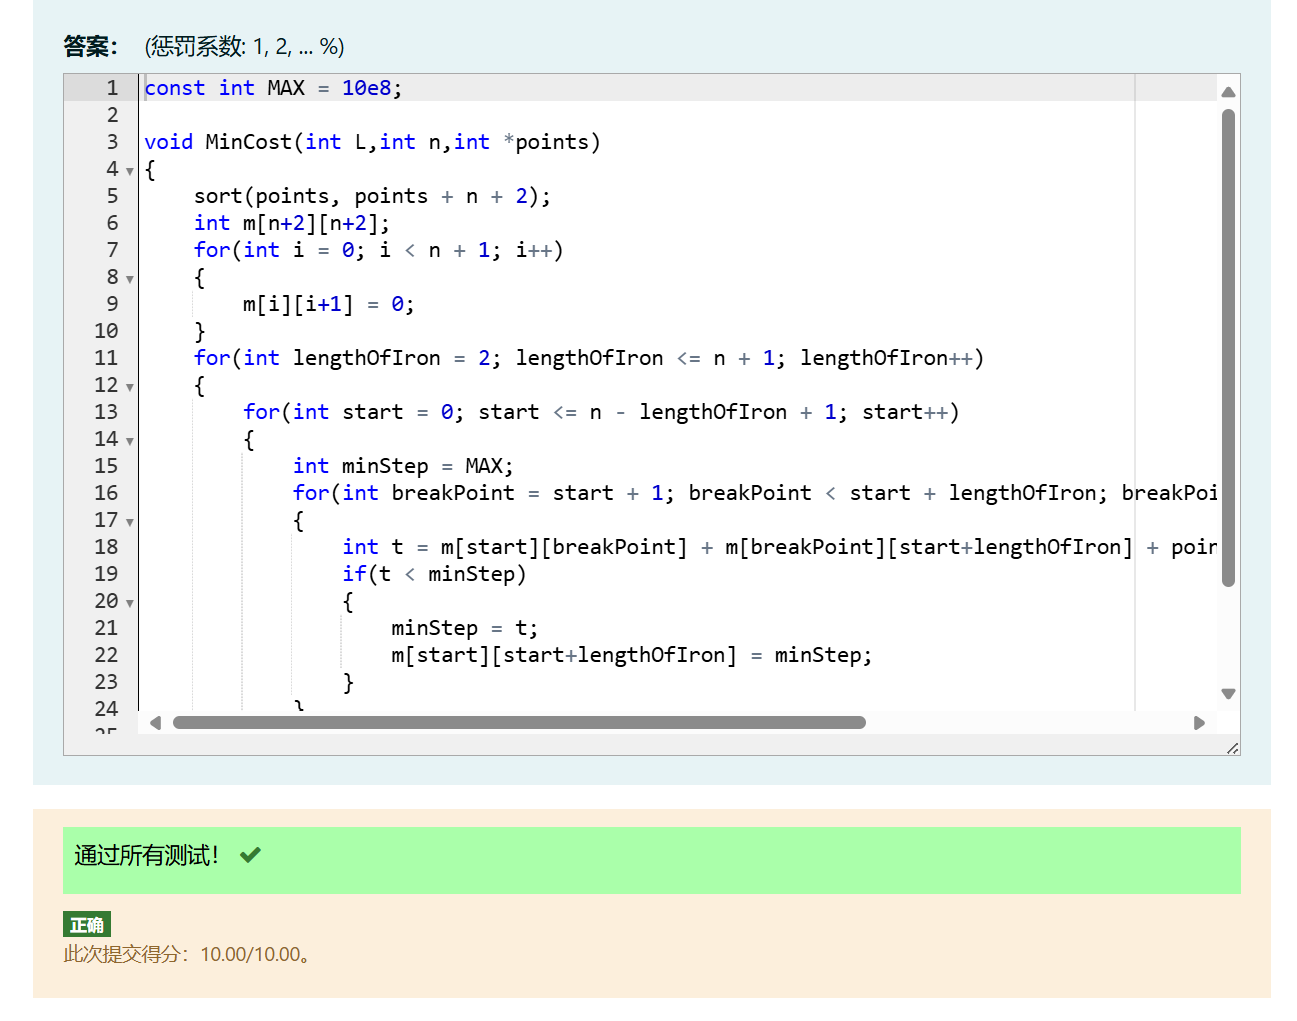
\includegraphics[width=0.8\textwidth]{moodle2.png}
\end{figure}

\section{反思与改进}
\subsection{反思}
初次提交时,没有考虑将minStep赋最大值,导致部分用例错误。此外,动规算法时间复杂度较高,当n值较大时,算法的效率明显下降。
\subsection{改进}
本算法可以通过四边形不等式和单调性条件进行优化.
注意到,本题目时间代价$w(a,b) = a - b$满足四边形不等式$w(a,c) + w(b,d) \leq w(a,d) + w(b,c), a \leq b \leq c \leq d$,
则本题满足单调性条件,在本问题中,即有假设对于子问题$dp[i][j]$,最优切割点是$k$,则对于更大的区间$dp[i][j+1]$其最优切割点不会小于k。
利用这个性质,可以将内层循环修改为
\begin{lstlisting}
int optimalK = (i < j - 1) ? s[i][j - 1] : i + 1;  // 初始切割点选择
for (int k = optimalK; k <= s[i + 1][j]; k++) //应用单调性条件
{
    int minStep = m[i][k] + m[k][j] + points[j] - points[i];
    if (minStep < m[i][j]) 
    {
        m[i][j] = minStep;
    }
}
\end{lstlisting}
如此优化,代码时间复杂度将降为$O(n^2)$
\end{document}